% $Id$
% ..............................................................................
%                      E n c r y p t i o n   M e t h o d s
% ~~~~~~~~~~~~~~~~~~~~~~~~~~~~~~~~~~~~~~~~~~~~~~~~~~~~~~~~~~~~~~~~~~~~~~~~~~~~~~


%% Remark: Mit \begin{bibunit}[unsrt]  hier w�rde ein Kapitel-Bibliography erzeugt, das
%%         Zahlen anzeigt und unsortiert ist. Die Reihenfolge ergibt dann sich anhand der
%%         Abfolge der Referenzen im Quelltext.
\begin{bibunit}[babalpha]  %% alpha: Kapitel-Bibliography zeigt Autorenk�rzel und ist auch danach
	                   %%     sortiert. Gleiches K�rzel wie in der zweiten Gesamtbibliography.


\hypertarget{Chapter_EncryptionSecDefinitions}{}

\chapter{Security Definitions and Encryption Procedures}
\label{Chapter_EncryptionSecDefinitions}
(\hyperlink{author_Bernhard-Esslinger}{Bernhard Esslinger},
 \hyperlink{author_Joerg-Cornelius-Schneider}{Joerg-Cornelius Schneider},
 May 1999; Updates Dec 2001, Feb 2003, Jun 2005, Jul 2007, Jan 2010, Mar 2013, Aug 2016)

This chapter introduces the topic in a more descriptive way without using too much mathematics.

The purpose of encryption \index{encryption} is to change data in such a way
that only an authorized recipient is able to reconstruct the plaintext. This
allows us to transmit data without worrying about it getting into unauthorized
hands. Authorized recipients possess a piece of secret information -- called the
key -- which allows them to decrypt the data while it remains hidden from
everyone else.\footnote{%
  However, an attacker still can disturbe the connection or tap metadata (like who
  is communicating with whom).
}

For explanations in the following we use the notation from 
Figure \ref{cm_Generic-Notations-when-Encrypting}:
\begin{figure}[ht]
\begin{center}
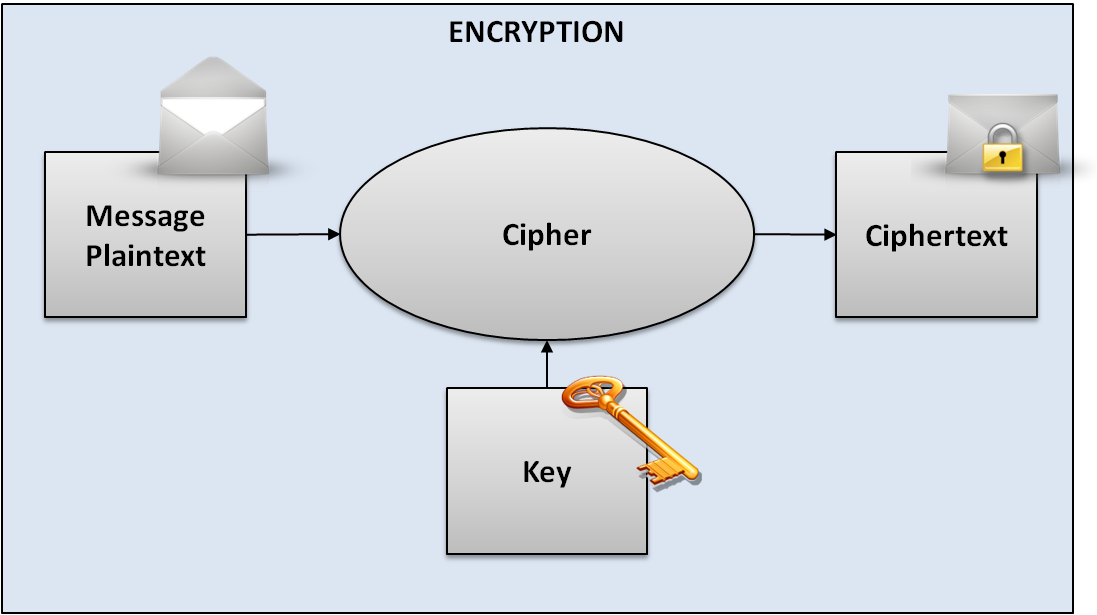
\includegraphics[scale=0.7]{figures/Generic-Notation-Encryption_en.png}
\caption{Common notations when using ciphers} 
\label{cm_Generic-Notations-when-Encrypting}
\end{center}
\end{figure}



% --------------------------------------------------------------------------
\newpage

\begin{ctsquote}
\caption{Saying from India}
Explain it to me, I will forget it.\\
Show it to me, maybe I will remember it.\\
Let me do it, and I will be good at it.
\end{ctsquote}

% --------------------------------------------------------------------------
\hypertarget{cm_Section_Security_Definitions}{}
% \section[Security definitions]{Security definitions}
\section{Security definitions and the importance of cryptology}
\label{cm_Section_Security_Definitions}
\index{security definitions}

First we present the ideas how the security of cryptosystems is defined.

Modern cryptography is heavily based on mathematical theory and computer
science practice. Cryptographic algorithms are designed around computational
hardness assumptions, making such algorithms hard to break in practice by any
adversary.

\vskip +3pt
Depending on the adversary's capabilities there are mainly two basic notations
of security distinguished in literature
(see e.g. {\em Contemporary Cryptography} \cite{Oppliger2011}):

\begin{itemize}

\item {\bf Computational, conditional or practical security}\\
  A cipher is {\em computationally} secure if it is theoretically possible to break
  such a system but it is infeasible to do so by any known practical means. Theoretical
  advances (e.g., improvements in integer factorization algorithms) and faster
  computing technology require these solutions to be continually adapted. 

  Even using the best known algorithm for breaking it will require so much
  resources (e.g., 1,000,000 years) that practically the cryptosystem is secure.

  So this concept is based on assumptions of the adversary's limited computing
  power and the current state of science.

\item {\bf Information-theoretical or unconditional security}\\
  A cipher is considered {\em unconditionally} secure if its security is guaranteed
  no matter how much resources (time, space) the attacker has -- so even in the case
  where the adversary has unlimited resources for breaking a cipher. Even with
  unlimited resources an adversary is unable to gain any meaningful data from a
  ciphertext.

  There exist information-theoretically secure schemes that provably cannot be
  broken even with unlimited computing power -- an example is the
  {\em one-time pad} (OTP\index{OTP}).

  As the OTP is information-theoretically secure it derives its security
  solely from information theory and is secure even with unlimited computing
  power at the adversary's disposal. However, OTP has several practical
  disadvantages (the key used must be used only once, randomly selected and must
  be at least as long as the message being protected), which means that it is
  hardly used except in closed environments such as for the hot wire between
  Moscow and Washington.%\par \vskip + 3pt

\end{itemize}


\vskip +3pt
\noindent Two more concepts are sometimes used:

\begin{itemize}

\item {\bf Provable security}
This means that breaking such a cryptographic system is as difficult as
solving some supposedly difficult problem e.g. discrete logarithm computation,
discrete square root computation, very large integer factorization.

Example: Currently we know that RSA\index{RSA} is at most as difficult as
factorization, but we cannot prove that its exactly as difficult as
factorization.
So RSA has no proven minimum security. Or in other words: We cannot prove,
that if RSA (the cryptosystem) is broken, that then factorization (the hard
mathematical problem) can be solved.

The Rabin cryptosystem was the first cryptosystem which could be proven to be
computationally equivalent to a hard problem.

\item {\bf Ad-hoc security}
A cryptographic system has this security feature if it is not worth to try to
break into such a system because of inadequate price of data with comparison to
price of work needed to do so. Or an attack can't be done in sufficiently short
time (see {\em Handbook of Applied Cryptography} \cite{Menezes2001}).

Example: This may apply if a message relevant for the stock market will be
published tomorrow and you need a year to break it.

\end{itemize}


\vskip +3pt
For good procedures used today the time taken to break them is so long that
it is practically impossible to do so, and these procedures can therefore be
considered (practically) secure -- from a pure algorithm's point of view.\footnote{%
  Especially after the knowledge gathered by Edward Snowden\index{Snowden, Edward}
  there were many discussions,
  whether encryption is secure. In \cite{Esslinger2014} is the result of an evaluation,
  which cryptographic algoritms can be relied on -- according to current knowledge.
  The article investigates: Which crypto systems can -- despite the reveal of
  the NSA/GCHQ attacks -- still be considered as secure? Where have systems
  been intentionally weakened? How can we create a secure cryptographic future?
  Where is the difference between maths and implementation?
}

\vskip +3pt
We basically distinguish between symmetric
(see chapter \ref{cm_Section_Symmetric-encryption}) and asymmetric
(see chapter \ref{cm_Section_Asymmetric-encryption}) encryption
procedures.
The books of Bruce Schneier \cite{Schneier1996} and Klaus Schmeh
\cite{Schm2016} also offer a very good overview of the different
encryption algorithms.\footnote{%
  A compact overview about what is used where, which methods are secure, where you
  have to anticipate problems and where the construction areas will be in the
  future (incl. the lengthy procedures of the standardization) can be found in
  the German article \cite{Schmidt2016}.
}

\vskip +3pt
With the use of the internet and wireless communication, encryption technologies
are used (mostly transparently) by everyone. However, they have been in use since
centuries by governments, military, and diplomats. The side which had a better command
of these technologies could exert big influence on {\bf politics} and war with the help
of secret services.
This book only touches history when introducing the earlier cipher methods in
chapter \ref{Chapter_PaperandPencil}. You can gain an impression, how important
cryptology was and still is, by considering the following two examples: the
educational film ``War of the letters'' (German: Krieg der Buchstaben)\footnote{%
  See \url{http://bscw.schule.de/pub/bscw.cgi/d1269787/Krieg_der_Buchstaben.pdf}.\\
  A supporting quote from Denis Smyth, professor in the Department of History
  and the International Relations Programme at the University of Toronto:
  ``Secret intelligence has long been regarded as the ``missing dimension'' of
  international relations.'' (from \url{http://www.secretintelligencefiles.com})
}
and the debates around the so called crypto wars\footnote{%
  See \url{https://en.wikipedia.org/wiki/Crypto_Wars}.\index{crypto wars}
}.



% --------------------------------------------------------------------------
\newpage

\begin{ctsquote}
``One cannot not communicate.''
\caption[Paul Watzlawick]{Paul Watzlawick\footnotemark}\index{Watzlawick, Paul}
\end{ctsquote}
\addtocounter{footnote}{0}\footnotetext{Paul Watzlawick, Janet H. Beavin, and Don D. Jackson, ``Pragmatics of human communication; a study of interactional patterns, pathologies, and paradoxes'', Norton, 1967, The first of five axioms of their human communications theory.}

% --------------------------------------------------------------------------
\section[Influences on encryption methods]{Influences on encryption methods}

\nopagebreak
Here, we just want to mention two aspects often neglected and dealt with too late:

\begin{itemize}

\item {\bf Random based}\\
\index{random}
Algorithms can be divided up into deterministic\index{deterministic} and heuristic\index{heuristic} methods. Most students only learnt deterministic methods, where the output is uniquely determined by the input. On the other hand, heuristic methods make decisions using random values. Modern methods of machine learning are also part of them.

Random looms large in cryptographic methods. Keys have to be selected randomly, which means that at least for the key generation ``random'' is necessary. In addition, some methods, especially from cryptanalysis, are heuristic.

\item {\bf Constant based}\\
Many modern methods (especially hash methods and symmetric encryption) use numeric constants. Their values should be plausible and they shouldn't contain back doors. Numbers fulfilling this requirement are called nothing-up-my-sleeve numbers\index{number!nothing-up-my-sleeve}.%
\footnote{\url{http://en.wikipedia.org/wiki/Nothing_up_my_sleeve_number}}

\end{itemize}


\newpage
The following figure \ref{cm_Figure_OTP-demo-pictures} intends to give an idea, that it is impossible to determine the correct plaintext from a OTP\index{OTP} (if the OTP method has been applied correctly and if all keys have the same likelyhood).

The example in this figure uses an 8 character long given ciphertext:
\texttt{11 1B 1E 18 00 04 0A 15}.
There are many meaningful words with 8 letters and for each there is an according key.
So an attacker can not determine alone from the ciphertext, which is the correct key and which is the correct plaintext word.

Also see figure~\ref{fig-bool-otp} in chapter~\ref{s-bool-bitstr-real-random},
where an according example with text strings is build with SageMath.
\begin{figure}[ht]
\begin{center}
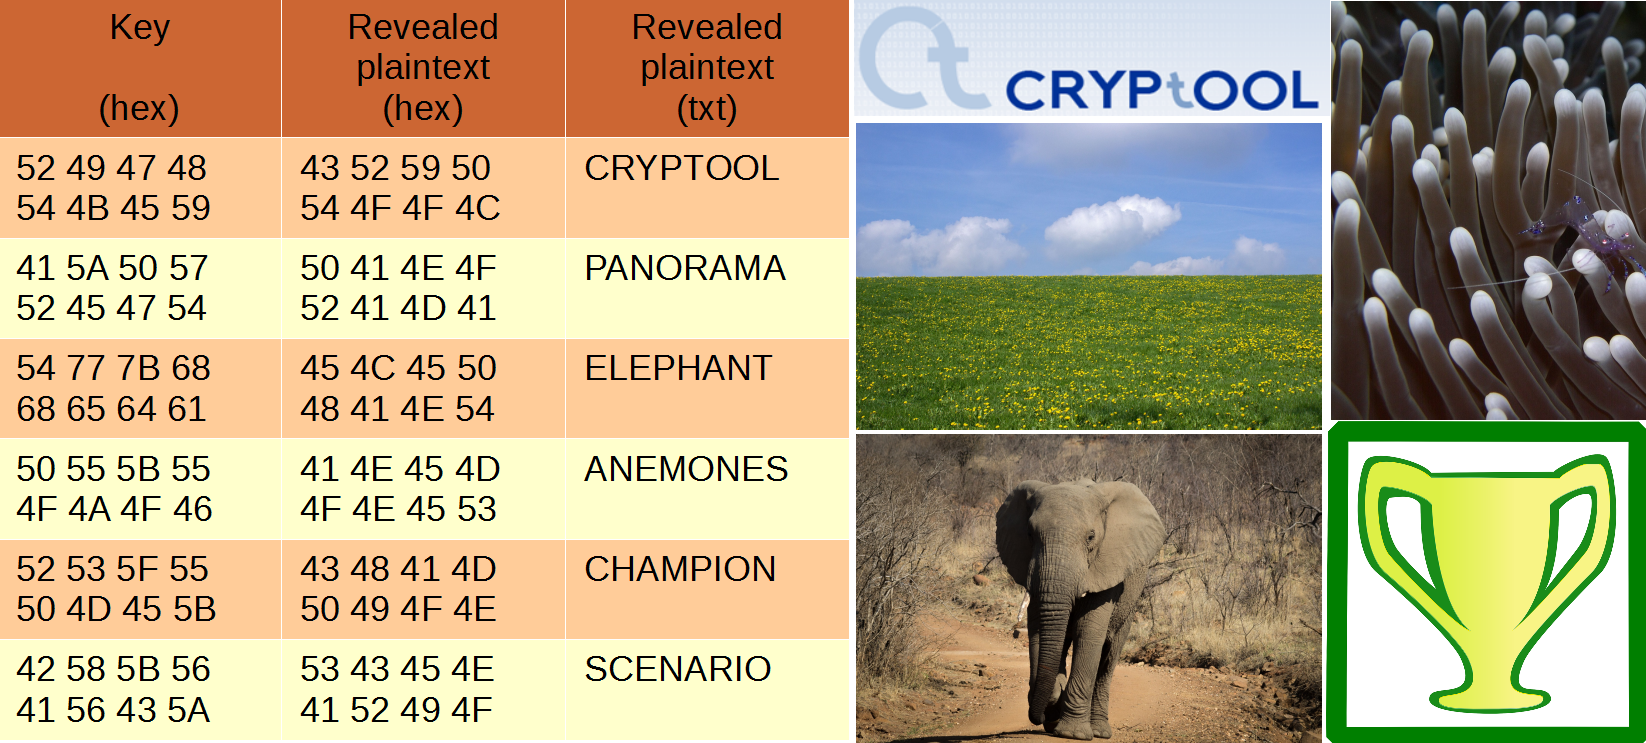
\includegraphics[scale=0.54]{figures/OTP-demo-pictures-en.png}
\caption[Illustration for the information-theoretically secure OTP scheme]
        {Illustration for the information-theoretically secure OTP scheme\footnotemark}
\label{cm_Figure_OTP-demo-pictures}
\end{center}
\end{figure}
\footnotetext{
  Picture source: Free pictures from \url{https://pixabay.com/}
}





% --------------------------------------------------------------------------
\newpage

\begin{ctsquote}
``Transparency. That's the best one can hope for in a technologically advanced society ... otherwise you will just be manipulated.''
\caption[Daniel Suarez]{Daniel Suarez\footnotemark}\index{Suarez, Daniel}
\end{ctsquote}
\addtocounter{footnote}{0}\footnotetext{Daniel Suarez, ``Freedom'',
   Dutton Adult, 2010, Chapter 5, ``Getting with the Program'', p. 63, Price.}

% --------------------------------------------------------------------------
\section[Symmetric encryption]
        {Symmetric encryption\footnotemark}
  \footnotetext{%
    With CrypTool~1 ({\bf CT1})\index{CT1} you can execute
    the following modern symmetric encryption algorithms 
    (using the menu path {\bf Crypt \textbackslash{} Symmetric (modern)}):\\
    IDEA, RC2, RC4, DES (ECB), DES (CBC), Triple-DES (ECB), Triple-DES (CBC),
    MARS (AES candidate), RC6 (AES candidate), Serpent (AES candidate), 
    Twofish (AES candidate), Rijndael (official AES algorithm)\index{AES}.\\
    With CrypTool~2 ({\bf CT2})\index{CT2} you can execute the
    following modern symmetric encryption algorithms (using in the Startcenter
    {\bf Templates
    \textbackslash{} Cryptography \textbackslash{} Modern \textbackslash{}
    Symmetric}):\\
    AES, DES, PRESENT, RC2, RC4, SDES, TEA, Triple-DES, Twofish.\\
    In JCrypTool ({\bf JCT})\index{JCT} you can execute the
    following modern symmetric encryption algorithms:\\ 
    AES, Rijndael, Camellia, DES, Dragon, IDEA, LFSR, MARS, Misty1, RC2, RC5,
    RC6, SAFER+, SAFER++, Serpent, Shacal, Shacal2, Twofish.
  }
\label{cm_Section_Symmetric-encryption}

\nopagebreak
For {\em symmetric} encryption \index{encryption!symmetric} sender and
recipient must be in possession of a common (secret) key which they have
exchanged before actually starting to communicate. The sender uses this
key to encrypt the message and the recipient uses it to decrypt it.
\par %\vskip + 3pt

This is visualized in Figure \ref{cm_Figure_Symmetric-Enc_Secret-Key-Enc}:
\begin{figure}[ht]
\begin{center}
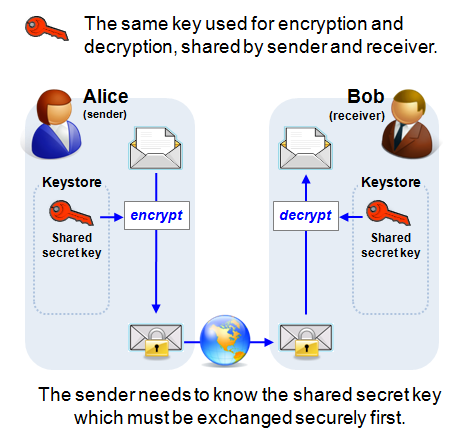
\includegraphics[scale=0.7]{figures/SymmetricEnc_Figure_Chap1_en.png}
\caption{Symmetric or secret-key encryption} 
\label{cm_Figure_Symmetric-Enc_Secret-Key-Enc}
\end{center}
\end{figure}

All classical ciphers are of the type symmetric. Examples can be found within
the CT programs, in chapter~\ref{Chapter_PaperandPencil}
(``\nameref{Chapter_PaperandPencil}'')
of this script, or in \cite{Nichols1996}.
In this section however, we want to consider only modern symmetric mechanisms.

The advantages of symmetric algorithms are the high speed with which data can be
encrypted and decrypted. One disadvantage is the need for key management. In
order to communicate with one another confidentially, sender and recipient must
have exchanged a key using a secure channel before actually starting to
communicate. Spontaneous communication between individuals who have never met
therefore seems virtually impossible. If everyone wants to communicate with
everyone else spontaneously at any time in a network of $ n $ subscribers, each
subscriber must have previously exchanged a key with each of the other $n - 1$
subscribers. A total of $n(n - 1)/2$ keys must therefore be exchanged.\par \vskip + 3pt



\subsection[AES (Advanced Encryption Standard)]{AES (Advanced Encryption Standard)\footnotemark} 
\footnotetext{%
   In CT1\index{CT1} you can find 3 visualizations for this cipher via
   the menu {\bf Indiv. Procedures \textbackslash{} Visualization of
   Algorithms \textbackslash{} AES}.\\
   In CT2\index{CT2} you can find a template performing AES step-by-step
   (by entering the search string ``AES'' in the Startcenter).
}
\label{CM_AES}
\index{AES}

Before AES, the most well-known modern symmetric encryption procedure was the
DES\index{DES} algorithm.
The DES algorithm has been developed by IBM in collaboration with the
National Security Agency \index{NSA} (NSA), and was published as a standard in
1975. Despite the fact that the procedure is relatively old, no effective attack
on it has yet been detected. The most effective way of attacking consists of
testing (almost) all possible keys until the right one is found ({\em brute-force-attack}).
\index{attack!brute-force} Due to the relatively short key length of
effectively 56 bits (64 bits, which however include 8 parity bits), numerous
messages encrypted using DES have in the past been broken. Therefore, the
procedure can not be considered secure any longer. Alternatives to the DES
procedure include IDEA\index{IDEA}, Triple-DES (TDES) and especially AES.
\par \vskip + 3pt

Up-to-the-minute procedure for symmetric ciphers is the AES\index{AES}. The associated
Rijndael algorithm was declared winner of the AES award on October 2nd, 2000
and thus succeeds the DES procedure.\index{AES}

An introduction and further references about the AES algorithms and the AES
candidates of the last round can be found i.e. within the online help of
CrypTool\index{CrypTool}%
\footnote{%
      CrypTool~1 online help\index{CT1}: The index head-word {\bf AES}
      leads to the 3 help pages: {\bf AES candidates}, 
      {\bf The AES winner Rijndael} and 
      {\bf The Rijndael encryption algorithm}\\
      A comprehensive description of AES including C code can be found
      in \cite{Haan2008}.
  }
oder in Wikipedia%
\footnote{%
	\url{https://en.wikipedia.org/wiki/Advanced_Encryption_Standard}
  }.



\clearpage
\noindent The two screenshots \ref{AES-Visualization-Zabala-Flash-step3} and
\ref{AES-Visualization-Zabala-Flash-step5} are taken from one of three
AES visualizations in CT1\index{CT1}.

\begin{figure}[!ht]
\begin{center}
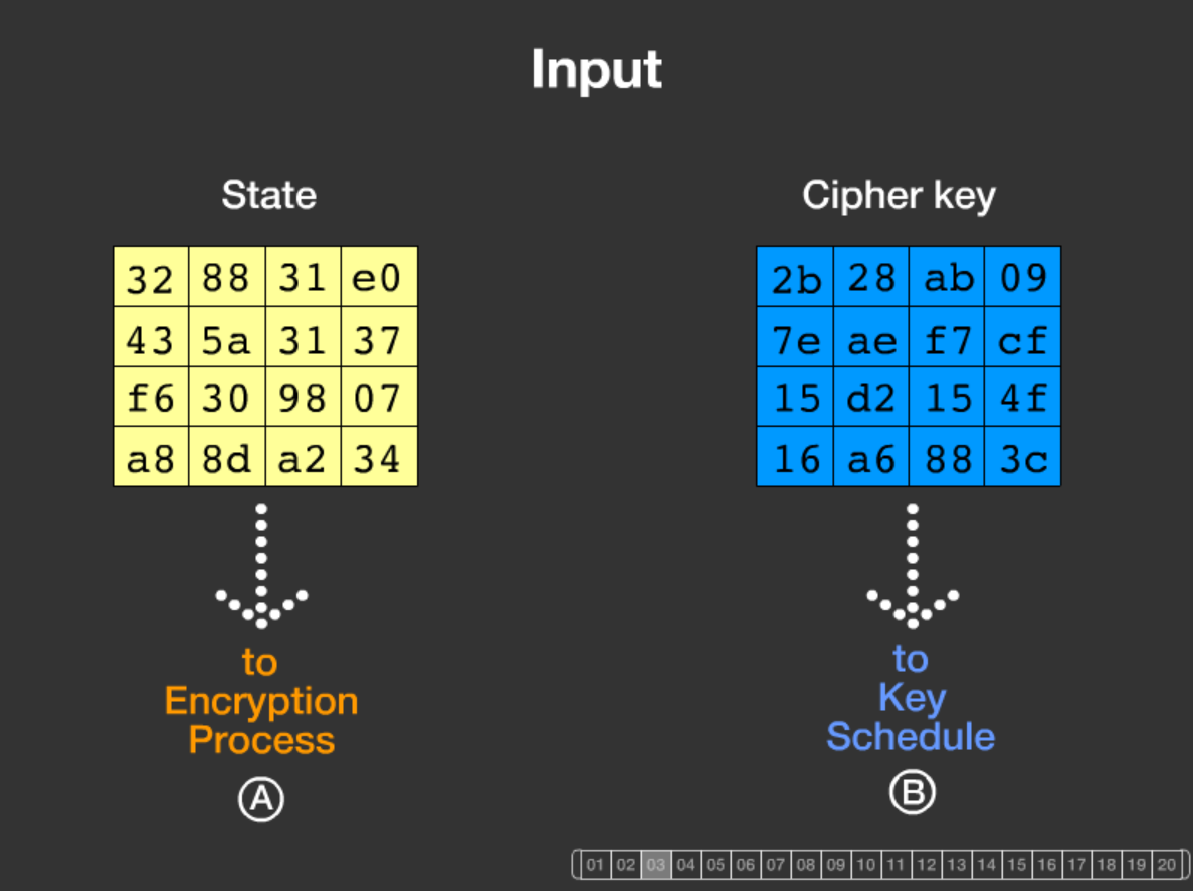
\includegraphics[scale=0.6]{figures/AES-Visualization-Zabala-Flash-step3_en}
\caption{AES visualization by Enrique Zabala from CT1 (part 1)}
\label{AES-Visualization-Zabala-Flash-step3}
\end{center}
\end{figure}

\begin{figure}[!ht]
\begin{center}
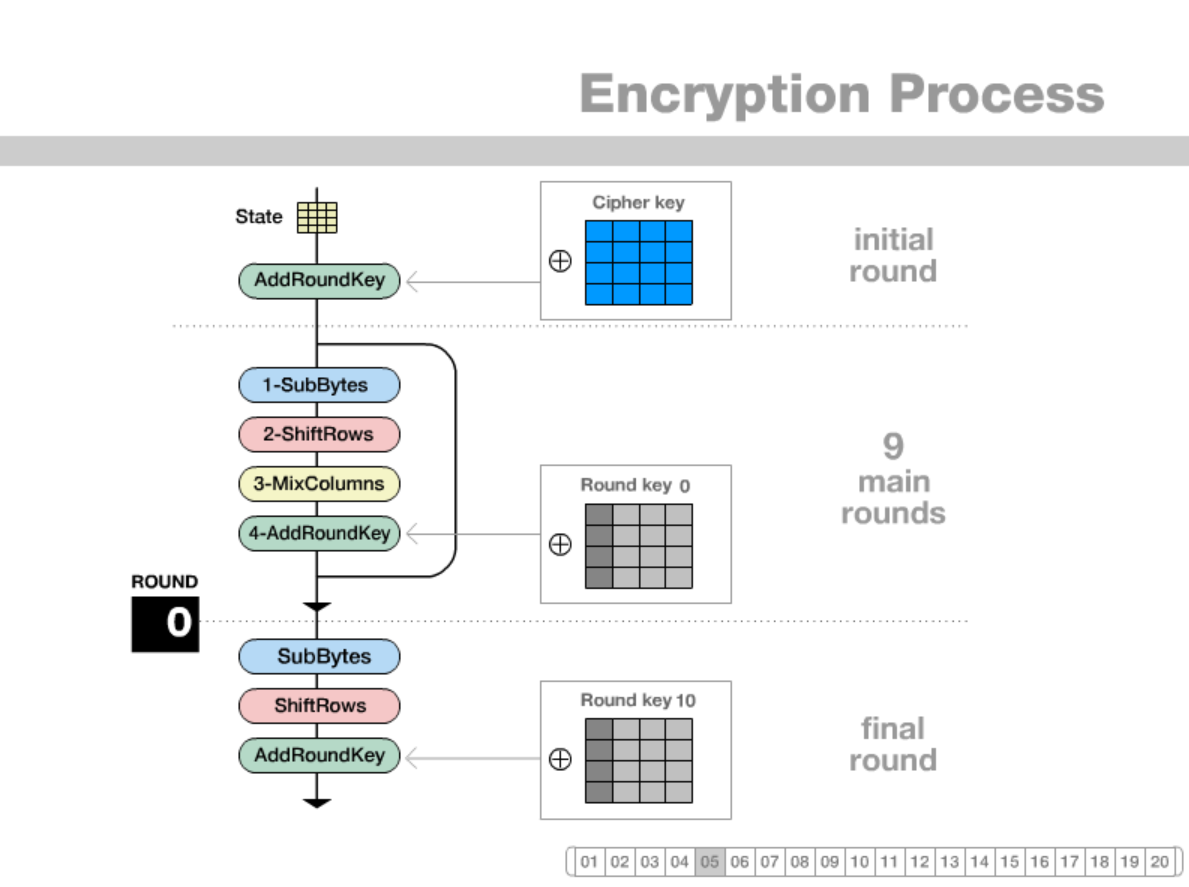
\includegraphics[scale=0.6]{figures/AES-Visualization-Zabala-Flash-step5_en}
\caption{AES visualization by Enrique Zabala from CT1 (part 2)}
\label{AES-Visualization-Zabala-Flash-step5}
\end{center}
\end{figure}
%\end{sloppypar}


\clearpage
\noindent Now we want to encrypt with AES in CBC mode a 128-bit block of plaintext.
Off the resulting ciphertext we are only interested in
the 1st block (if there is more, it would be padding, here null-padding).
For demonstration we do it once with CT2 and once with OpenSSL.\\

\noindent Figure \ref{AES_Encrypting-one-block-with-CT2} shows the encryption of
one block in {\bf CT2}\index{CT2}.

\noindent The plaintext ``AESTEST1USINGCT2'' is converted to hex
(41 45 53 54 45 53 54 31 55 53 49 4E 47 43 54 32). Using this and the key
3243F6A8885A308D313198A2E0370734 the AES component creates the ciphertext.
It is in hex:\\
B1 13 D6 47 DB 75 C6 D8 47 FD 8B 92 9A 29 DE 08

\begin{figure}[ht]
\begin{center}
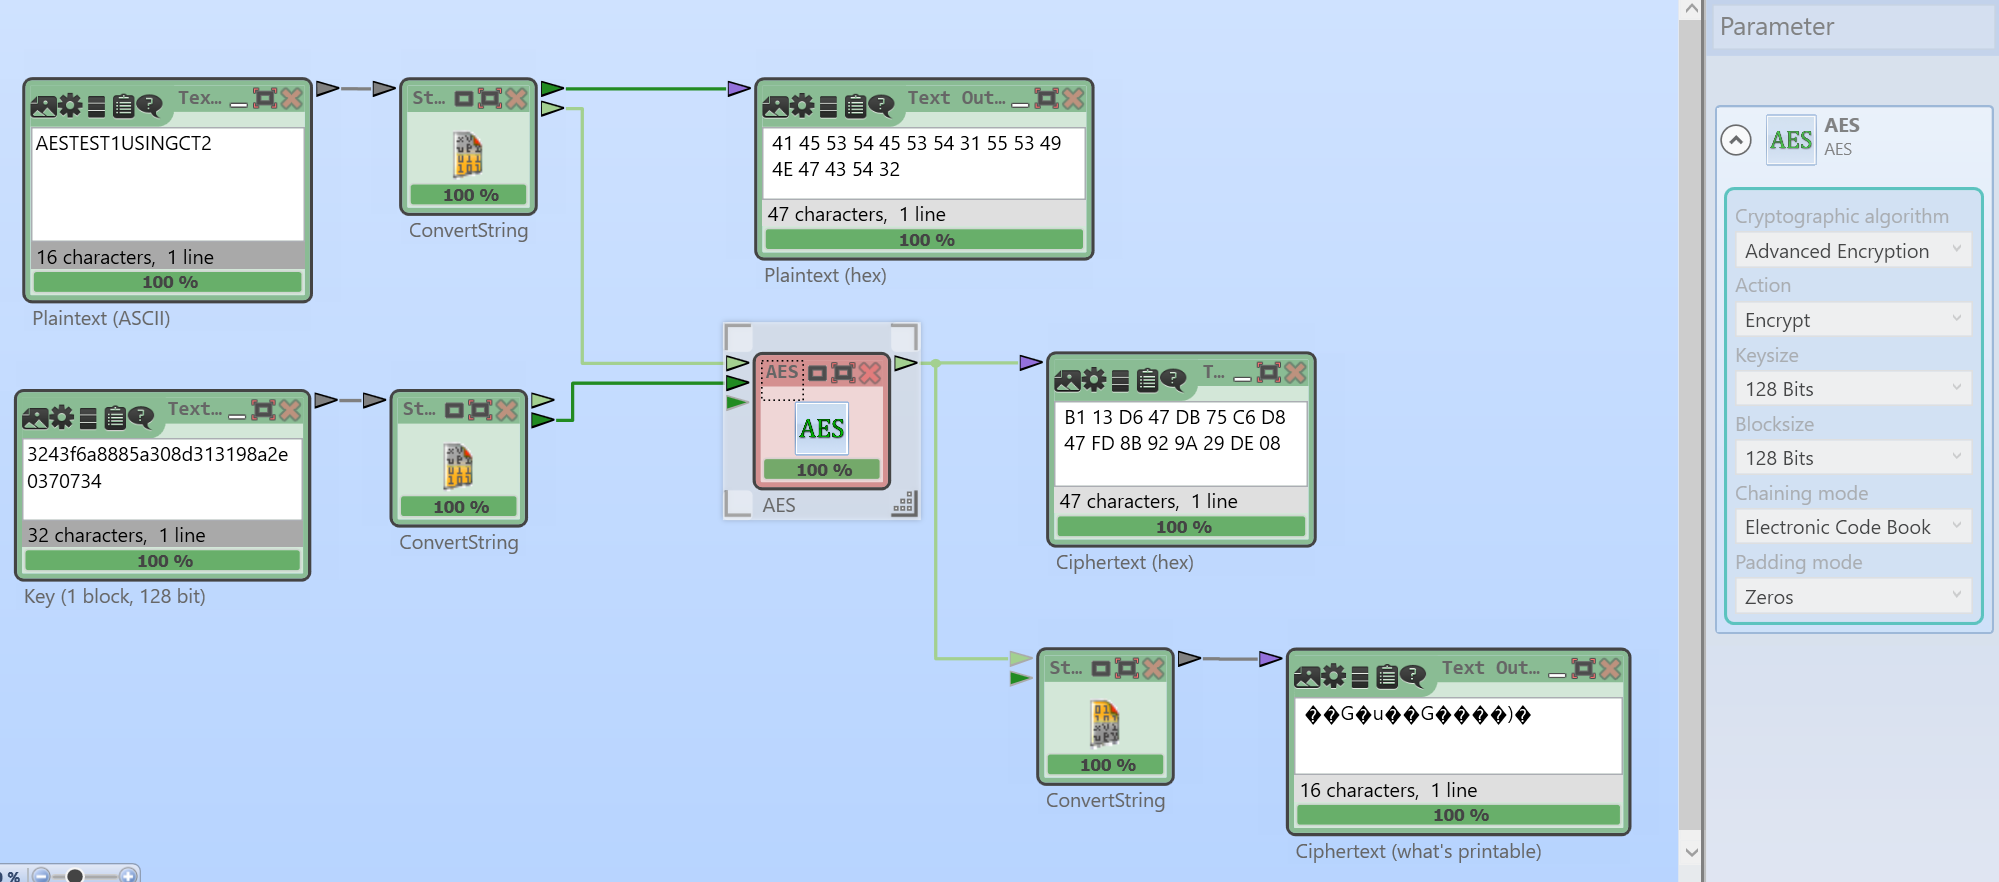
\includegraphics[scale=0.42]{figures/AES_Encrypting-one-block-with-CT2_en}
\caption{AES encryption (of exactly 1 block and without padding) in CT2} 
\label{AES_Encrypting-one-block-with-CT2}
\end{center}
\end{figure}


\vspace{15pt}
\noindent The same result can be achieved with {\bf OpenSSL}\index{OpenSSL}%
\footnote{%
      OpenSSL\index{OpenSSL} is a very widespread free open-source crypto library,
      used by many applications, for instance to implement the TLS protocol.
      Part of OpenSSL is the commandline tool openssl, which can be used to test
      the functionality directly on many operating systems and to request, create
      and manage certificates.\\
      Contrarily to the also very widespread and very good commandline tool gpg from
      GNU Privacy Guard\index{GnuPG}
      (\url{https://en.wikipedia.org/wiki/GNU_Privacy_Guard}),
      openssl also allows calls with many details.
      The gpg has its focus on the practically applied ciphersuites.
      As far as we know, it is not possible to encrypt just one block without padding
      with the commandline tool gpg.\\
      Also see \url{https://en.wikipedia.org/wiki/OpenSSL}.
  }
from the commandline:
\begin{opensslcode}
\begin{Verbatim}%
[fontsize=\footnotesize]
>openssl enc -e -aes-128-cbc
        -K 3243F6A8885A308D313198A2E0370734
        -iv 00000000000000000000000000000000
        -in klartext-1.hex  -out klartext-1.hex.enc
>dir
06.07.2016  12:43                16 key.hex
20.07.2016  20:19                16 klartext-1.hex
20.07.2016  20:37                32 klartext-1.hex.enc
\end{Verbatim}
\caption{AES encryption (of exactly one block and without padding) in OpenSSL}
\label{cm_AES_no-padding:OpenSSL_example}
\end{opensslcode}





\clearpage
% HACK to fix warning "destination with the same identifier .. has already been used, ...":
%\makeatletter \renewcommand{\thepage}{\csname @arabic\endcsname \c@page} \makeatother
% --------------------------------------------------------------------------
\subsubsection{Results about theoretical cryptanalysis of AES}
\label{cm_New-AES-Analysis}
\index{cryptanalysis}
\index{AES}

Below you will find some results, which have recently called into question the security of the AES algorithm -- from our point of view these doubts practically still remain unfounded
% = do not bring disrepute upon AES
. 
The following information is based particularly on the original papers and the
articles \cite{Wobst2002} and \cite{Lucks2002}.

AES with a minimum key length of 128 bit is still in the long run sufficiently secure against brute-force attacks\index{attack!brute-force} -- as long as the quantum computers aren't powerful enough. When announced as new standard AES was immune against all known cryptanalytic attacks, mostly based on statistical considerations and earlier applied to DES: using pairs of clear and cipher texts expressions are constructed, which are not completely at random, so they allow conclusions to the used keys. These attacks required unrealistically large amounts of intercepted data.

Cryptanalysts already label methods as ``academic success'' or as ``cryptanalytic attack'' if they are theoretically faster than the complete testing of all keys (brute force analysis). In the case of AES with the maximal key length (256 bit) exhaustive key search on average needs $2^{255}$ encryption operations. A cryptanalytic attack needs to be better than this. At present between $2^{75}$ and $2^{90}$ encryption operations are estimated to be performable only just for organizations, for example a security agency.

In their 2001-paper Ferguson, Schroeppel and Whiting \cite{Ferguson2001}
presented a new method of symmetric codes cryptanalysis: They described AES with
a closed formula (in the form of a continued fraction) which was possible
because of the ``relatively'' clear structure of AES. This formula consists of
around 1000 trillion terms of a sum - so it does not help concrete practical
cryptanalysis. Nevertheless curiosity in the academic community was awakened.
It was already known, that the 128-bit AES could be described as an
over-determined system of about 8000 quadratic equations (over an algebraic
number field) with about 1600 variables (some of them are the bits of the wanted
key) -- equation systems of that size are in practice not solvable. This special
equation system is relatively sparse, so only very few of the quadratic terms
(there are about 1,280,000 are possible quadratic terms in total) appear in the
equation system.

The mathematicians Courtois and Pieprzyk \cite{Courtois2002} published a paper
in 2002, which got a great deal of attention amongst the cryptology community: The
pair had further developed the XL-method (eXtended Linearization), introduced at
Eurocrypt 2000 by Shamir et al., to create the so called XSL-method (eXtended
Sparse Linearization). The XL-method is a heuristic technique, which in some
cases manages to solve big non-linear equation systems and which was till then
used to analyze an asymmetric algorithm (HFE).  The innovation of Courtois and
Pieprzyk was, to apply the XL-method on symmetric codes: the XSL-method can be
applied to very specific equation systems. A 256-bit AES could be attacked in
roughly $2^{230}$ steps. This is still a purely academic attack, but also a
direction pointer for a complete class of block ciphers. The major problem with
this attack is that until now nobody has worked out, under what conditions it is
successful: the authors specify in their paper necessary conditions, but it is
not known, which conditions are sufficient.  There are two very new aspects of
this attack: firstly this attack is not based on statistics but on algebra. So
attacks seem to be possible, where only very small amounts of ciphertext are
available. Secondly the security of a product algorithm%
\index{product algorithm}\index{encryption!product algorithm}%
\index{cascade cipher}\index{encryption!cascade cipher}%
\footnote{%
A ciphertext can be used as input for another encryption algorithm. 
A cascade cipher%
\index{product algorithm}\index{encryption!product algorithm}%
\index{cascade cipher}\index{encryption!cascade cipher}%
is build up as a composition of different encryption transformations.
The overall cipher is called product algorithm or cascade cipher
(sometimes depending whether the used keys are statistically dependent or not).\\
Cascading does not always improve the security.\\
This process is also used {\em within} modern algorithms:
They usually combine simple and, considered at its own, cryptologically
relatively insecure single steps in several rounds into an efficient 
overall procedure.  Most block ciphers (e.g. DES, IDEA) are cascade ciphers.\\
Also serial usage of the same cipher with different keys (like with Triple-DES)
is called cascade cipher.\index{DES!Triple-DES}
}
does not exponentially increase with the number of rounds.

Currently there is a large amount of research in this area: for example Murphy and Robshaw presented a paper at Crypto 2002 \cite{Robshaw2002a}, which could dramatically improve cryptanalysis: the burden for a 128-bit key was estimated at about $2^{100}$ steps by describing AES as a special case of an algorithm called BES (Big Encryption System), which has an especially ``round'' structure. But even $2^{100}$ steps are beyond what is achievable in the foreseeable future. Using a 256 bit key the authors estimate that a XSL-attack will require $2^{200}$ operations.

More details can be found in the Web links section at
\hyperlink{CM_HT_Weblink_Rijndael-Cryptosystem}{``AES or Rijndael cryptosystem''}.

So for AES-256 the attack is much more effective than brute-force\index{attack!brute-force}
but still far away from any computing power which could be accessible in the short-to-long term. 

The discussion temporarily was very controversial: Don Coppersmith (one of the
inventors of DES) for example queries the practicability of the attack because
XLS would provide no solution for AES \cite{Coppersmith2002}. This implies that
then the optimization of Murphy and Robshaw \cite{Robshaw2002b} would not work.

In 2009 Biryukov and Khovratovich \cite{Biryukov2009} published another
theoretical attack on AES. This attack uses different methods from the ones
described above. They applied methods from hash function cryptanalysis (local
collisions and boomerang switching) to construct a related-key attack on
AES-256. I.~e.\ the attacker not only needs to be able to encrypt arbitrary data
(chosen plain text), in addition he needs to be able to manipulate the unknown key
(related-key). 

Based on those assumptions, the effort to find a AES-256 key is reduced to
$2^{119}$ time and $2^{77}$ memory (considering asymmetric complexity).
In the case of AES-192 the attack is even less practical, for AES-128
the authors do not provide an attack.


% --------------------------------------------------------------------------
\subsection{Algebraic or algorithmic cryptanalysis on symmetric algorithms}
\index{attack!algebraic}
\index{SAT solver}
\label{cm_Algebraic-versus-Symmetr}

There are different modern methods attacking the structure of a problem directly or after a transformation of the problem. One of the attack methods is based on the satisfiability problem (SAT)%
\footnote{%
  \url{http://en.wikipedia.org/wiki/Boolean_satisfiability_problem}
}.


%\vskip +25 pt
\paragraph*{Description of a SAT solver}\index{SAT solver}\mbox{}
\hypertarget{ht_SAT-Solver}{}

An old and well-studied problem in computer science is called the SAT problem. Here, for a given Boolean formula, it's the task to find out whether there is an assignment of the variables, so that the evaluation result of the formula is 1. 

Example: The Boolean formula ``A AND B'' evaluates to 1, if and only if A=B=1. For the formula ``A AND NOT(A)'' there exists no assignment of its variable A, so that the formula is evaluated to the value 1.

For larger Boolean formulas, it is not easy to determine if an assignment exists for which the formula can be evaluated to 1 (this problem belongs to the NP-complete problems). Therefore specific tools have been developed to solve this problem for general Boolean formulas, so called SAT solvers\footnote{
    With {\bf CT2}\index{CT2} you can execute
    a SAT solver -- using in the Startcenter
    {\bf Templates
    \textbackslash{} Mathematics \textbackslash{}
    SAT Solver (Text Input)}  and  {\bf SAT Solver (File Input)}.
    }. As has been found, SAT solvers can also be used to attack cryptographic systems.


%\vskip +25 pt
\paragraph*{SAT solver based cryptanalysis}\index{SAT solver}\mbox{}
\hypertarget{ht_SAT-Solver_Cryptanalysis}{}

The general approach to use SAT solvers in cryptanalysis is very straightforward: First, the cryptographic problem, e.g. finding the symmetric key or an inversion of a hash function, is translated into a SAT problem. Then, the SAT solver can be used to find a solution to the SAT problem. The solution of the SAT problem then also solves the original cryptographic problem.
The paper by Massacci \cite{Massacci2000} describes the first known usage of a SAT solver in this context. Unfortunately, very soon it turned out that such a general approach cannot be used efficiently in practice. This is due to the fact that the cryptographic SAT problems are very complex and the runtime of a SAT solver increases exponentially with the problem size. Therefore, in modern approaches SAT solvers are used only for solving partial problems of cryptanalysis. A good example for this is described in the paper by Mironov and Zhang \cite{Mironov2006}. They demonstrate the usage of a SAT solver in an attack on hash functions, where the SAT solver is used to solve some partial problems in a very efficient way.



% --------------------------------------------------------------------------
\subsection{Current status of brute-force attacks on symmetric algorithms}
\index{attack!brute-force}
\index{RC5}
\label{cm_Brute-force-versus-Symmetr}

The current status of brute-force attacks on symmetric encryption algorithms can be explained with the block cipher RC5.

Brute-force (exhaustive search, trial-and-error) means to completely examine all keys of the key space: so no special analysis methods have to be used. Instead, the ciphertext is decrypted with all possible keys%
\footnote{%
    With CT1\index{CT1} you can also perform brute-force attacks
    of modern symmetric algorithms (using the menu path
    {\bf Analysis \textbackslash{} Symmetric Encryption (modern)}): Here
    the weakest knowledge of an attacker is assumed, he performs a 
    ciphertext-only attack.\\
    With CT2\index{CT2} you can also perform brute-force attacks
    (using the templates under {\bf Cryptanalysis \textbackslash{} Modern}).
    Highly powerful is the KeySearcher component, which can be used to
    distribute the calculations to many different computers.
}
and for each resulting text it is checked, whether this is a meaningful clear text%
\footnote{%
    If the cleartext is written in a natural language and at least 100 B
    long, this check also can be performed automatically.\\
    To achieve a result in an appropriate time with a single PC you should 
    mark not more than 24 bit of the key as unknown.
}.
A key length of 64 bit means at most $2^{64}$ = 18,446,744,073,709,551,616
or about 18 trillion (GB) / 18 quintillion (US)  keys to check\index{CrypTool}.

Companies like RSA Security provided so-called cipher challenges\index{challenge}
in order to quantify the security offered by well-known symmetric ciphers as DES,
Triple-DES or RC5%
\index{DES}\index{RC5}\index{DES!Triple-DES}.%
\footnote{%
  \url{https://www.emc.com/emc-plus/rsa-labs/historical/the-rsa-laboratories-secret-key-challenge.htm}\\
  Unfortunately, in May 2007 RSA Inc announced that they will not confirm the
  correctness of the not yet solved RC5-72 challenge.

  There are also cipher challenges for asymmetric algorithms (please see
  chapter \ref{nt:NoteFactorization}).

  A wide spectrum of both simple and complex, both symmetric and asymmetric crypto riddles
  are included in the international cipher contest {\bf MysteryTwister C3}:
  \url{http://www.mysterytwisterc3.org}.
  \index{MTC3}\index{crypto challenge}
}
They offered prizes for those who managed to decipher ciphertexts, encrypted
with different algorithms and different key lengths, and to unveil the symmetric
key (under controlled conditions). So theoretical estimates can be confirmed.

It is well-known, that the ``old'' standard algorithm DES with a fixed key
length of 56 bit is no more secure: This was demonstrated already in January
1999 by the Electronic Frontier Foundation (EFF). With their specialized
computer Deep Crack they cracked a DES encrypted message within less than a
day.\footnote{%
  \url{https://www.emc.com/emc-plus/rsa-labs/historical/des-challenge-iii.htm}
}

The current record for strong symmetric algorithms unveiled a key 64 bit long.
The algorithm used was RC5, a block cipher with variable key size. 

The RC5-64 challenge has been solved in July 2002 by the distributed.net team
after 5 years.\footnote{%
  \url{http://www.distributed.net/Pressroom_press-rc5-64}\\
  \url{http://www.distributed.net/images/9/92/20020925_-_PR_-_64_bit_solved.pdf}
% The pdf is the former page
%  \url{http://distributed.net/pressroom/news-20020926.html}
}
In total 331,252 individuals co-operated over the internet to find the
key.\footnote{%
An overview of current distributed computing projects can be found here:\\
\url{http://distributedcomputing.info/}
}
More than 15 trillion (GB) / 15 quintillion (US)  keys were checked, until they
found the right key.%
\footnote{%
  CT2\index{CT2} started to experiment with a general infrastructure for
  distributed computing called CrypCloud\index{CrypCloud} (both peer-to-peer and
  centralized). So in the future, CT2 will be able to distribute the calculations
  on many computers. What could be achieved
  after the components are made ready for parallelization showed a cluster for
  distributed cryptanalysis of DES and AES: Status on March 21st, 2016 is,
  that an AES brute-force attack (distributed keysearching) worked on
  50 i5 PCs, each with 4 virtual CPU cores. These 200 virtual ``worker threads'' 
  achieved to test about 350 million AES keys/sec. The ``cloud'' processed a total
  amount of about 20 GB/sec of data. CrypCloud is a volunteering cloud system
  which enables CT2 users to voluntarily join distributed computing jobs. 
}


So, symmetric algorithms (even if they have no cryptographic weakness)
using keys of size 64 bit are no more appropriate to keep sensible data private.



% --------------------------------------------------------------------------
\newpage
\section[Asymmetric encryption]
{Asymmetric encryption\footnotemark}
  \footnotetext{%
    The RSA cryptosystem can be executed in many variations with 
    CT1\index{CT1} (using the menu path
    {\bf Individual Procedures \textbackslash{} RSA Cryptosystem \textbackslash{}
    RSA Demonstration}).\\
    With CT1\index{CT1} you can execute RSA encryption and decryption
    (using the menu path {\bf Crypt \textbackslash{} Asymmetric}).
    In both cases you must select a RSA key pair. Only in the case of decryption
    the secret RSA key is necessary -- so here you are asked to enter the PIN.\\
    With CT2\index{CT2} you can also perform asymmetric methods
    (using the templates under {\bf Cryptography \textbackslash{} Modern}).\\
    JCT\index{JCT} offers asymmetric methods like RSA both within
    the {\bf Visuals} menu of the Default Perspective as well as within the
    Algorithm Perspective.
  }
\label{cm_Section_Asymmetric-encryption}

\nopagebreak
In the case of {\em asymmetric} encryption \index{encryption!asymmetric} each
subscriber has a personal pair of keys consisting of a {\em secret}
\index{key!secret} key and a {\em public} key\index{key!public}. The public
key, as its name implies, is made public -- e.g. in a key directory on the
Internet (this kind of ``bill-board'' is also called just directory or
public key ring) or within a so-called public-key \index{certificate}
certificate.\par \vskip + 3pt

The asymmetric encryption is visualized in Figure \ref{cm_Figure_Asymmetric-Enc_Public-Key-Enc}:
\begin{figure}[ht]
\begin{center}
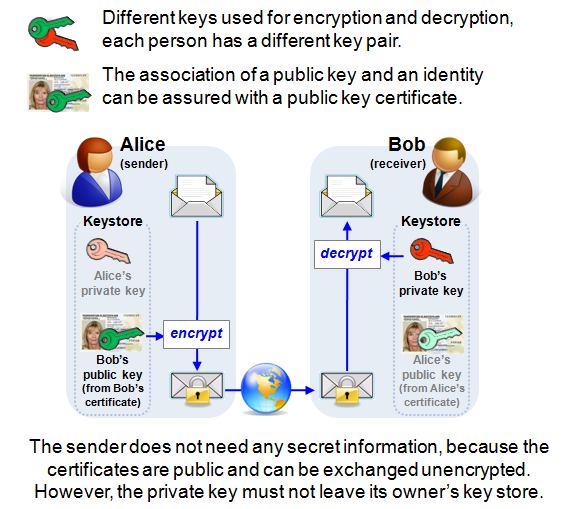
\includegraphics[scale=0.7]{figures/AsymmetricEnc_Figure_Chap1_en.png}
\caption{Asymmetric or public-key encryption} 
\label{cm_Figure_Asymmetric-Enc_Public-Key-Enc}
\end{center}
\end{figure}

If Alice\index{Alice}%
\footnote{%
      In order to describe cryptographic protocols participants
      are often named Alice, Bob\index{Bob}, \dots (see \cite[p. 23]{Schneier1996}). 
      Alice and Bob perform all 
      2-person-protocols. Alice will initiate all protocols and 
      Bob answers. The attackers are named Eve (eavesdropper) and
      Mallory (malicious active attacker).
  } wants to communicate with Bob, then she looks for Bob's public key 
and uses it to encrypt her message to him. She then sends
this ciphertext to Bob, who is then able to decrypt it again using his 
secret key. As only Bob knows his secret key, only he can decrypt 
messages addressed to him.
Even Alice who sends the message cannot restore plaintext from the (encrypted)
message she has sent. Of course, you must first ensure that the public key
cannot be used to derive the private key.\par \vskip + 3pt

% Abbildung evtl. besser hier, wenn Seitenaufteilung ausginge.

Such a procedure can be demonstrated using a series of thief-proof letter boxes.
If I have composed a message, I then look for the letter box\index{letter box}
of the recipient and post the letter through it. After that, I can no longer
read or change the message myself, because only the legitimate recipient has
the key for the letter box.\par \vskip + 3pt

The advantage of asymmetric procedures is the easier \index{key management}
key management. Let's look again at a network with $n$
subscribers. In order to ensure that each subscriber can establish
an encrypted connection to each other subscriber, each subscriber
must possess a pair of keys. We therefore need $2n$ keys or $n$
pairs of keys. Furthermore, no secure channel is needed before
messages are transmitted, because all the information required in
order to communicate confidentially can be sent openly. In
this case, you simply\footnote{%
That this is also not trivial is explained e.g. in chapter
\ref{nt_Shared-Primes}.
Besides the requirements for the key generation it has to be considered that
nowadays also (public-key) infrastructures itself are targets of cyber attacks.
}
have to pay attention to the accuracy
(integrity and authenticity) \index{authenticity} of the public
key. Disadvantage: Pure asymmetric procedures take a lot longer to
perform than symmetric ones.\par \vskip + 3pt

The most well-known asymmetric procedure is the \index{RSA} 
RSA algorithm\index{CrypTool}%
\footnote{%
  The RSA algorithm is extensively described in chapter \ref{rsabeweis} and later
  within this script. 
  The topical research results concerning RSA are described 
  in chapter \ref{SecurityRSA}.
}%
, named after its developers Ronald \index{Rivest, Ronald} Rivest, Adi
\index{Shamir, Adi} Shamir and Leonard \index{Adleman, Leonard} Adleman.
The RSA algorithm was published in 1978.\footnote{%
  Hints about the history of RSA and its publication which didn't amuse the NSA
  can be found within the series {\em RSA \& Co. at school: Modern cryptology, old
  mathematics, and subtle protocols}.
  Unfortunately these are currently only available in German.
  See \cite{Witten2006}, pp 55 ff (``Penible L�mmergeier'').
  \index{RSA \& Co. at school}
}
The concept of asymmetric encryption was first
introduced by Whitfield Diffie \index{Diffie, Whitfield}  and Martin
\index{Hellman, Martin} Hellman in 1976. Today, the ElGamal \index{ElGamal,
Tahir} procedures also play a decisive role, particularly the \index{Schnorr,
Claus-Peter} Schnorr variant in the \index{DSA} DSA \index{signature!digital}
(Digital Signature Algorithm).

\noindent Attacks against asymmetric ciphers are touched in\\
- chapter~ \ref{Chapter_ElementaryNT}: \hyperlink{Chapter_ElementaryNT}{Elementary Number Theory},\\
- chapter~ \ref{Chapter_ModernCryptography}:
  \hyperlink{Chapter_ModernCryptography}{Modern Cryptography},\\
- chapter~ \ref{Chapter_EllipticCurves}:
  \hyperlink{Chapter_EllipticCurves}{Elliptic Curves}, and\\
- chapter \ref{Chapter_Dlog-FactoringDead}: \hyperlink{Chapter_Dlog-FactoringDead}
  {Current Results for Solving Discrete Logarithms And Factoring}.



% --------------------------------------------------------------------------
\newpage
\section[Hybrid procedures]{Hybrid procedures\footnotemark}
\footnotetext{%
   Within CT1\index{CT1} you can find this technique using the menu
   path {\bf Crypt \textbackslash{} Hybrid}: 
   There you can follow the single steps and its dependencies with concrete
   numbers. The variant with RSA as the asymmetric algorithm is graphically
   visualized; the variant with ECC uses the standard dialogs. In both cases
   AES is used as the symmetric algorithm.\index{AES}\\
   JCT\index{JCT} offers hybrid methods like ECIES within
   the Algorithm Perspective under {\bf Algorithms \textbackslash{} Hybrid Ciphers}.
}%
\label{CM_Hybrid-procedures}
\index{hybrid procedure}

In order to benefit from the advantages of symmetric and asymmetric
techniques together, hybrid procedures \index{encryption!hybrid} are
usually used (for encryption) in practice. \par \vskip + 3pt

In this case the bulk data is encrypted using symmetric procedures: The key
used for this is a secret session key\index{session key} generated by the
sender randomly\footnote{%
   An important part of cryptographically secure techniques is to generate 
   random numbers\index{random}.\\
   - Within CT1\index{CT1} you can check out different random number
   generators\index{random generator} (PRNGs) using the menu path
   {\bf Indiv. Procedures \textbackslash{} Generate Random Numbers}. 
   Using the menu path {\bf Analysis \textbackslash{} Analyze Randomness}
   you can apply different test methods for random data to binary documents. \\
   % CT1 concentrates on cryptographically strong {\bf pseudo} random number
   % generators. ``Real'' random sources are only included via calling the
   % integrated Secude generator.\\
   %
   - In CT2\index{CT2} you can find templates using 
   PRNGs (by entering the search string ``random'' in the Startcenter).
   The PRNGs\index{random generator} internally use for instance
   Keccak\index{Keccak} or the Linear
   Congruential Generator (LCG)\index{LCG}, and they are used e.g. for
   key generation or decimalization.\\
   %
   - JCT\index{JCT} offers {\bf pseudo} random number generators both
   within the Default Perspective in the menu {\bf Algorithms \textbackslash{}
   Random Number Generator} as well as within the Algorithm Perspective.
}\index{random}
that is only used for this message.

This session key is then encrypted using the asymmetric procedure, and
transmitted to the recipient together with the message.

Recipients can determine the session key using their private keys and
then use the session key to encrypt the message.

In this way, we can benefit from the easy key management\index{key management}
of asymmetric procedures (using public/private keys) and we benefit from the
efficiency of symmetric procedures to encrypt large quantities of data
(using secret keys).



% --------------------------------------------------------------------------
\newpage

\begin{ctsquote}
    There is an old saying inside the US National Security Agency (NSA):\\
    ``Attacks always get better; they never get worse.''
\caption[IETF]{IETF\footnotemark}
\end{ctsquote}
\addtocounter{footnote}{0}\footnotetext{%
  \url{http://tools.ietf.org/html/rfc4270}\index{IETF}\index{NSA}
  }

% --------------------------------------------------------------------------
\section[Cryptanalysis and symmetric ciphers for educational purposes]{Cryptanalysis and symmetric ciphers for educational purposes\footnotemark}
\footnotetext{%
  A very good starting point to learn cryptanalysis is the book from Mark
  Stamp \cite{Stamp2007}. 
  Also good, but very high-level and concentrating on analyzing symmetric block ciphers
  only, is the article from Bruce Schneier \cite{Schneier2000}.\\
  Several of the cipher challenges at ``MysteryTwister C3''
  (\url{http://www.mysterytwisterc3.org}) are also well suitable for educational purposes.
  \index{MTC3}\index{crypto challenge}
}
\label{CM_Analysis-SymCiphers-Educational}
\index{cryptanalysis}

Compared to public-key ciphers based on mathematics like RSA, the structure of AES\index{AES} and most other modern symmetric ciphers (like DES, IDEA or Present), is very complex and cannot be explained as easily as RSA\index{RSA}.

So simplified variants of modern symmetric ciphers were developed for
educational purposes in order to allow beginners to perform
encryption and decryption by hand and gain a better understanding of how the
algorithms work in detail.
These simplified variants also help to understand and apply the according
cryptanalysis methods.

The most well-known of these variants are SDES (Simplified DES)%
\footnote{
  If you double-click on the title of the icon of the SDES component in CT2\index{CT2}
  you can see a visualization of the SDES algorithm, showing how the bits of the
  given data flow through the whole algorithm. An according screenshot:
  \url{https://www.facebook.com/CrypTool2/photos/a.505204806238612.1073741827.243959195696509/597354423690316}
}
and S-AES (Simplified-AES) by Prof. Ed Schaefer and his students%
\footnote{
    See the article ``Devising a Better Way to Teach and Learn the
    Advanced Encryption Standard'' at
    \url{http://math.scu.edu/~eschaefe/getfile.pdf}
},
and Mini-AES (see chapter~\ref{CM_Sage_Mini-AES} ``\nameref{CM_Sage_Mini-AES}''):

\index{DES}\index{DES!SDES}\index{IDEA}\index{AES!Mini-AES}\index{AES!S-AES}
\begin{itemize}

\item Edward F. Schaefer: {\em A Simplified Data Encryption Standard Algorithm} 
      \cite{Schaefer1996}.

\item Raphael Chung-Wei Phan: {\em Mini Advanced Encryption Standard (Mini-AES):
                                   A Testbed for Cryptanalysis Students} 
      \cite{Phan2002}.

\item Raphael Chung-Wei Phan: {\em Impossible differential cryptanalysis of Mini-AES} 
      \cite{Phan2003}.

\item Mohammad A. Musa, Edward F. Schaefer, Stephen Wedig:
      {\em A simplified AES algorithm and its linear and differential cryptanalyses} 
      \cite{Musa2003}.

\item Nick Hoffman: {\em A SIMPLIFIED IDEA ALGORITHM} 
      \cite{Hoffman2006}.

\item S. Davod. Mansoori, H. Khaleghei Bizaki: 
      {\em On the vulnerability of Simplified AES Algorithm Against Linear Cryptanalysis} 
      \cite{Mansoori2007}.

\end{itemize}




% --------------------------------------------------------------------------
\section{Further information}

Beside the information you can find in the following chapters, in many other
books and on a good number of websites, the online help of all
CrypTool variants\index{CrypTool} also offer very many details about the 
symmetric and asymmetric encryption methods.


	

% ---------------------------------------------------------------------------
% ---------------------------------------------------------------------------
\newpage
\hypertarget{CM_Appendix_SageCode}{}
\section{Appendix: Examples using SageMath}
\label{CM_Sage_samples}
\index{SageMath!code examples}

\noindent Below is SageMath source code related to contents of the
chapter~\ref{CM_Analysis-SymCiphers-Educational}
(``\nameref{CM_Analysis-SymCiphers-Educational}''). 

Further details concerning cryptosystems within SageMath (e.g. about the Simplified
Data Encryption Standard SDES) can be found e.g. in the thesis of Minh Van
Nguyen \cite{Nguyen2009b}.

% ---------------------------------------------------------------------------
\subsection{Mini-AES}
\label{CM_Sage_Mini-AES}
\index{AES!mini-AES}

The SageMath module \texttt{crypto/block\_cipher/miniaes.py} supports Mini-AES to allow
students to explore the inner working of a modern block cipher.

Mini-AES, originally described at \cite{Phan2002}, is a simplified variant of the
Advanced Encryption Standard (AES) to be used for cryptography education.

How to use Mini-AES is exhaustively described at the this SageMath reference page:
\begin{sloppypar}
  \url{http://doc.sagemath.org/html/en/reference/cryptography/sage/crypto/block_cipher/miniaes.html}.
\end{sloppypar}

The following SageMath code~\ref{cm_Mini-AES:Sage_example}
is taken from the release tour of SageMath 4.1%
\footnote{
  See \url{http://mvngu.wordpress.com/2009/07/12/sage-4-1-released/}.\\
  Further example code for Mini-AES can be found in
  \cite[chap. 6.5 and appendix D]{Nguyen2009a}.
}
and calls the implementation of the Mini-AES.


% Using [fontsize=\footnotesize,fontshape=tt] caused:
%   LaTeX Font Warning: Font shape `T1/cmtt/m/tt' undefined
%   (Font)              using `T1/cmtt/m/n' instead on input line 730.
% so deleted the fontshape parameter.
\begin{sagecode}
\begin{Verbatim}%
[fontsize=\footnotesize]
# We can encrypt a plaintext using Mini-AES as follows:
sage: from sage.crypto.block_cipher.miniaes import MiniAES
sage: maes = MiniAES()
sage: K = FiniteField(16, "x")
sage: MS = MatrixSpace(K, 2, 2)
sage: P = MS([K("x^3 + x"), K("x^2 + 1"), K("x^2 + x"), K("x^3 + x^2")]); P

[  x^3 + x   x^2 + 1]
[  x^2 + x x^3 + x^2]
sage: key = MS([K("x^3 + x^2"), K("x^3 + x"), K("x^3 + x^2 + x"), K("x^2 + x + 1")]); key

[    x^3 + x^2       x^3 + x]
[x^3 + x^2 + x   x^2 + x + 1]
sage: C = maes.encrypt(P, key); C

[            x       x^2 + x]
[x^3 + x^2 + x       x^3 + x]

# Here is the decryption process:
sage: plaintxt = maes.decrypt(C, key)
sage: plaintxt == P
True

# We can also work directly with binary strings:
sage: from sage.crypto.block_cipher.miniaes import MiniAES
sage: maes = MiniAES()
sage: bin = BinaryStrings()
sage: key = bin.encoding("KE"); key
0100101101000101
sage: P = bin.encoding("Encrypt this secret message!")
sage: C = maes(P, key, algorithm="encrypt")
sage: plaintxt = maes(C, key, algorithm="decrypt")
sage: plaintxt == P
True

# Or work with integers n such that 0 <= n <= 15:
sage: from sage.crypto.block_cipher.miniaes import MiniAES
sage: maes = MiniAES()
sage: P = [n for n in xrange(16)]; P
[0, 1, 2, 3, 4, 5, 6, 7, 8, 9, 10, 11, 12, 13, 14, 15]
sage: key = [2, 3, 11, 0]; key
[2, 3, 11, 0]
sage: P = maes.integer_to_binary(P)
sage: key = maes.integer_to_binary(key)
sage: C = maes(P, key, algorithm="encrypt")
sage: plaintxt = maes(C, key, algorithm="decrypt")
sage: plaintxt == P
True
\end{Verbatim}
\caption{Encryption and decryption with Mini-AES}
\label{cm_Mini-AES:Sage_example}
\end{sagecode}
\clearpage


% ---------------------------------------------------------------------------
\subsection{Further symmetric crypto algorithms in SageMath}
\label{CM_Sage_SymCryptoAlg}

The Reference for SageMath v7.2 lists e.g. the following further cryptographic functions:%
\footnote{
  See
  \url{http://doc.sagemath.org/html/en/reference/sage/crypto/index.html},\\
  \url{http://doc.sagemath.org/html/en/reference/cryptography/index.html}, and\\
  \url{http://combinat.sagemath.org/doc/reference/cryptography/sage/crypto/stream.html}
}
\begin{itemize}
   \item Linear feedback shift register (LFSR),
   \item Blum-Blum-Shub (BBS): pseudo-random generator (to be found with streams),
   \item Lattice-based functions.
\end{itemize}



%------------------------------------------------------------------------------
%%%%%\putbib[../de/references]
\putbib
\addcontentsline{toc}{section}{Bibliography}
\end{bibunit}

\noindent All links have been confirmed at July 10, 2016.



% --------------------------------------------------------------------------
\newpage
% \section*{Web links}\addcontentsline{toc}{section}{Web links}
\chapter*{Web Links}\addcontentsline{toc}{section}{Web Links}

\begin{enumerate}

  \hypertarget{CM_HT_Weblink_Rijndael-Cryptosystem}{}
  \item AES discussion groups at NIST (archive page provided for historical purposes, last update on Feb 28th, 2001)\\
	\url{http://csrc.nist.gov/archive/aes/}

  \item AES or Rijndael cryptosystem (page maintained by Nicolas T. Courtois, last update on Aug 24th, 2007)\\
        \url{http://www.cryptosystem.net/aes}

  \item distributed.net: ``RC5-64 has been solved''\\
        \url{http://www.distributed.net/Pressroom_press-rc5-64}

  \item RSA Labs (former RSA Security): ``The RSA Secret Key Challenge''
        \begin{sloppypar}
        \url{https://www.emc.com/emc-plus/rsa-labs/historical/the-rsa-laboratories-secret-key-challenge.htm}
	\end{sloppypar}

  \item RSA Labs (former RSA Security): ``DES Challenge''\\
        \url{https://www.emc.com/emc-plus/rsa-labs/historical/des-challenge-iii.htm}

  \item Further links can be found at the CrypTool homepage\\
        \url{http://www.cryptool.org}
	       
\end{enumerate}

All links have been confirmed at July 10, 2016.



% Local Variables:
% TeX-master: "../script-en.tex"
% End:
